\documentclass[accentcolor=tud2c,colorbacktitle,inverttitle,landscape,ngerman,presentation,t]{tudbeamer}
\usepackage{etex}
\usepackage{ngerman}
\usepackage[ngerman]{babel}
\usepackage[utf8]{inputenc}

\usepackage{pgfplots}
\pgfplotsset{compat=newest,
             grid=major}

\usepackage{tikz}
\usetikzlibrary{patterns}
\usetikzlibrary{calc,intersections,through,backgrounds}
\usepackage{multirow}
\usepackage{booktabs}
\usepackage{subcaption}
\usepackage{IEEEtrantools}


\begin{document}

\title[Fabelhafte Benner Boys]{Ableitung und Untersuchung des Abbruchfehlerschätzers für mittels
Finite Volumen diskretisierten Navier-Stokes Gleichungen}


\subtitle{Präsentation der Bachelor-Thesis}

\author{Paul Lange}
\institute{Institut für Numerische Berechnungsverfahren, TU Darmstadt}

%\logo{
\includegraphics{fnb_logo_schriftzug}}
\logo{
\includegraphics{fnblogo}}
% \logo{\color{tudtextaccent}\large IFP}

\date{\today}

\begin{titleframe}
\begin{figure}[h]
\centering
\vspace{10pt}
\begin{subfigure}[b]{.5\linewidth}
\centering
\begin{tikzpicture}
\begin{axis}[
view={150}{30},
xlabel=$x$,
ylabel=$y$,
height=150pt,
%zlabel={$f(x,y)$},
width=\textwidth
]
\addplot3[surf, mesh/ordering=y varies, faceted color=black] file{data/3/RES2_data.txt};
\end{axis}
\end{tikzpicture}
%\subcaption{Residuum}
\end{subfigure}%
\begin{subfigure}[b]{.5\linewidth}
\centering
\begin{tikzpicture}
\begin{axis}[
view={150}{30},
xlabel=$x$,
ylabel=$y$,
%zlabel={$f(x,y)$},
height=150pt,
width=\textwidth
]
\addplot3[surf, mesh/ordering=y varies, faceted color=black] file{data/3/TE2_data.txt};
\end{axis}
\end{tikzpicture}
%\subcaption{Abbruchfehler}
\end{subfigure}
%\caption{Residuum und Abbruchfehler ohne Randsprünge (Testfall 3)}
%\label{fig:t3_krand}
\end{figure}
\end{titleframe}


\begin{frame}
  \frametitle{\\Gliederung}
  \begin{itemize}
  \item Motivation
  \item Grundlagen
  \item Herleitung des Abbruchfehlerschätzers
  \item Verifikation des Abbruchfehlerschätzers
  \item Anwendung zur Gitteradaption
  \item Zusammenfassung
  \item Ausblick
  \end{itemize}
\end{frame}

\begin{frame}
  \frametitle{\\Motivation}
  \begin{itemize}
  \item Steigende Nutzung von CFD im Produktentwicklungsprozess
  \item Höhere Genauigkeit und größere Problemgebiete erforderlich
  \item Adaption des numerischen Gitters zur Verringerung der benötigten Rechenleistung
  \item Gitteradaption nach welchem Kriterium?
  \end{itemize}

  \begin{figure}
  \begin{center}
    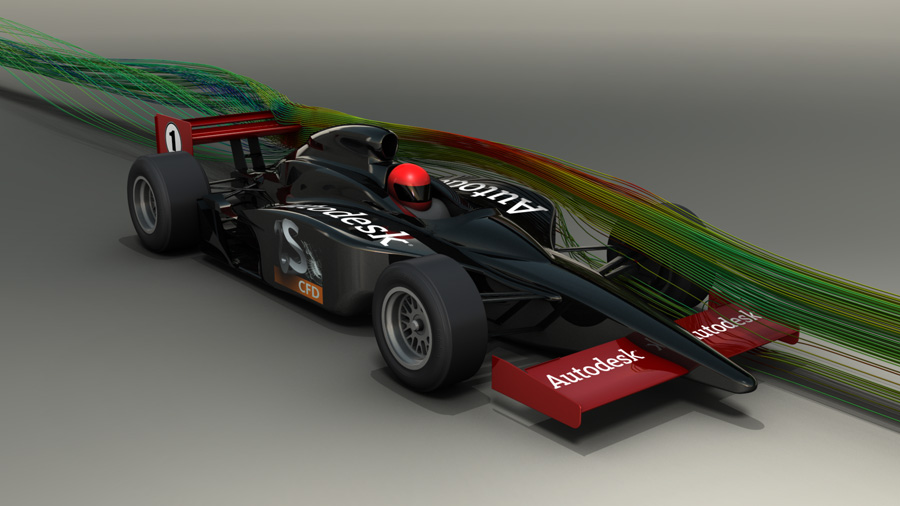
\includegraphics[scale=0.2]{auto}
  \end{center}
  \end{figure}
  \tiny Bildquelle: http://www.autodesk.de/adsk/servlet/pc/index?siteID=403786\&id=17361825
\end{frame}

\begin{frame}
  \frametitle{\\Allgemeine stationäre Transportgleichung}
    \begin{itemize}
      \item Herleitung anhand der allgemeinen Transportgleichung
  \end{itemize}
  \begin{equation*}
  \frac{\partial}{\partial x_i} \left({\rho v_i \phi
- \alpha \frac{\partial \phi}{\partial x_i} }\right) = f
\label{eq:transportgl}
\end{equation*}
\begin{itemize}
      \item Bei kleinen Reynoldszahlen gut auf Navier-Stokes-Gleichungen übertragbar
  \end{itemize}
\end{frame}


\begin{frame}
  \frametitle{\\Finite-Volumen Methoden}
    \begin{itemize}
      \item Standardverfahren zur Lösung von Strömungsproblemen
  \end{itemize}
\begin{align*}
    \frac{\partial}{\partial x_i} \left({\rho v_i \phi
    - \alpha \frac{\partial \phi}{\partial x_i} }\right) &= f\\
  \int_V \frac{\partial}{\partial x_i} \left({\rho v_i \phi
- \alpha \frac{\partial \phi}{\partial x_i} }\right) dV &= \int_V f dV \\
  \int_S  \left({\rho v_i \phi
- \alpha \frac{\partial \phi}{\partial x_i} }\right) n_i dS&= \int_V f dV \\
      \sum_c \int_{S_c} \left(\rho v_i \phi - \alpha \frac{\partial \phi}{\partial x_i}
      \right) n_{ci} dS_c &= \int_V f dV
\end{align*}
\end{frame}

\begin{frame}
  \frametitle{\\Finite-Volumen Methoden}
  \begin{figure}[ht]
  \begin{tikzpicture}[scale=0.8]
  \draw[->, thick] (-1.5,0) -- (-1,0) node[right] {$x$} coordinate(x axis);
  \draw[->, thick] (-1.5,0) -- (-1.5,0.5) node[above] {$y$} coordinate(y axis);

  \fill[tud0a] (0,1) -- (2,0.5) -- (2.5,2) -- (0.5, 3) --cycle;
  \draw[thick] (0,1) -- (2,0.5) -- (2.5,2) -- (0.5, 3) --cycle;
  \draw[thick] (4,-0.5) -- (2,0.5) -- (2.5,2) -- (5, 2.5) --cycle;

  %\fill (2,0.5,0) circle[radius=1.5pt];
  %\node (x) at (2,0.5) [label=below left:$se$] {};
  %\fill (2.5,2) circle[radius=1.5pt];
  %\node (x) at (2.5,2) [label=below right:$ne$] {};
  \fill (1.25,1.625) circle[radius=1.5pt];
  \node (x) at (1.25,1.625) [label=above:$P$] {};
  %\node (x) at (1.25,1.625) [label=below:{$(\xi_{i,j},\ \eta_{i,j})$}] {};
  \fill (3.25,1.125) circle[radius=1.5pt];
  \node (x) at (3.25,1.125) [label=above:$E$] {};
  %\node (x) at (3.25,1.125) [label=below:{$(\xi_{i+1,j},\ \eta_{i+1,j})$}] {};
  \fill (2.25,1.25) circle[radius=1.5pt];
  \node (x) at (2.25,1.25) [label=above left:$e$] {};

  %\draw[thick,->] (-0.75,2.125) -- (5.25,0.625);
  %\node (x) at (5.25,0.625) [label=right:$\xi$] {};

  %\draw[thick,->] (1.75,-0.25) -- (2.75,2.75);
  %\node (x) at (2.75,2.75) [label=right:$\eta$] {};
\end{tikzpicture}

\centering
%\caption{Berechnung der Metriken über Grenzen von Kontrollvolumen}
\end{figure}
    \begin{itemize}
      \item Approximation der Oberflächen- und Volumenintegrale
      \item Diskretisierung der konvektiven Flüsse
      \item Diskretisierung der diffusiven Flüsse
      \item Aufstellen des Gesamtgleichungssystems
    \end{itemize}
\end{frame}



\begin{frame}
  \frametitle{\\Abbruchfehler}
       \begin{itemize}
      \item  Fehler, der beim Abschneiden einer unendlichen Summe und deren Approximation durch
  eine endliche Summe entsteht.
      \item Bei FVM Diskretisierungen aus Taylorreihenentwicklungen hergeleitet
    \end{itemize}

    %\begin{block}{Beispiel}
      \begin{equation*}
  \sin(x) = \sum_{n=0}^{\infty}(-1)^n \frac{x^{2n+1}}{(2n+1)!} = 
  x-\frac{x^3}{3!} +\frac{x^5}{5!} -\frac{x^7}{7!} +\frac{x^9}{9!}+\cdots
 \label{eq:taylor_example}
\end{equation*}
\pause
\begin{align*}
  \sin(x) &\overset{!}{\approx} x-\frac{x^3}{3!}\\
  TE_{sin} &=  \frac{x^5}{5!} -\frac{x^7}{7!} +\frac{x^9}{9!}+\cdots\\
  \text{Fehlerschätzer} &=  \frac{x^5}{5!} -\frac{x^7}{7!}
\end{align*}
    %\end{block}
\end{frame}


\begin{frame}
  \frametitle{\\Abbruchfehler}
  \begin{itemize}
    \item Vergleich von Funktion und Approximation
  \end{itemize}
\begin{figure}[h]
\begin{tikzpicture}
\begin{axis}[width=0.9*\textwidth, height=170pt, grid=major,
  xlabel=$x$, ylabel=$f(x)$]
  \addplot[domain=-2*pi:2*pi, samples=100, color=tud2c, very thick]{sin(deg(x))};
  \addplot[domain=-3:3, samples=100, color=tud9c, very thick]{x - x*x*x/6};
  %, mark=triangle*, mark repeat=5
  \legend{$\sin(x)$,$x-\frac{x^3}{6} $}
\end{axis}
\end{tikzpicture}
\centering
%\caption{Vergleich von Funktion und Approximation}
 \label{fig:taylor_example}
\end{figure}
\end{frame}

\begin{frame}
  \frametitle{\\Abbruchfehler}
  \begin{itemize}
    \item Vergleich des absoluten Fehlers mit der Fehlerapproximation
  \end{itemize}
\begin{figure}[h]
\begin{tikzpicture}
\begin{axis}[width=0.9*\textwidth, height=170pt, grid=major, legend pos=north west,
  xlabel=$x$, ylabel=$f(x)$]
  \addplot[domain=-5:5, samples=100, color=tud2c, very thick]{sin(deg(x))-x+x*x*x/6};
  \addplot[domain=-6:6, samples=100, color=tud9c, very thick]{x^5/120-x^7/(120*6*7)};
  \legend{Absoluter Fehler, Fehlerapproximation}
\end{axis}
\end{tikzpicture}
\centering
%\caption{Vergleich des absoluten Fehlers mit der Approximation}
 \label{fig:taylor_example_te}
\end{figure}
\end{frame}


\begin{frame}
  \frametitle{\\Verifikation von Lösungsprogrammen}
    \begin{itemize}
      \item Nachweis der Korrektheit des numerischen Algorithmus
      \item Konvergenzordnung: Zusammenhang zwischen
        Verringerung des Diskretisierungsfehlers und Verfeinerung des numerischen Gitters
      \item Vergleich von
      \begin{itemize}
        \item Formaler Konvergenzordnung
          \begin{equation*}
            f''_i = \frac{f_{i+1}-2f_i +f_{i-1}}{\Delta x^2} -\frac{1}{12} f^{(4)}_i \Delta x^2 + HOT
\end{equation*}
        \item Beobachteter Konvergenzordnung
          \begin{equation*}
            DE_k=f(\Delta_k) - f_{exakt} = g_p h_k^{\tilde{p}} + HOT
\end{equation*}
\begin{equation*}
  \tilde{p}=\frac{\ln \left(DE_2/DE_1\right)}{\ln \left(h_2 / h_1\right)}
  \label{eq:beobachtet}
\end{equation*}
      \end{itemize}
    \end{itemize}
\end{frame}


\begin{frame}
  \frametitle{\\Verifikation der Lösungsprogramme}
  \only<1>{
    \begin{itemize}
      \item Eindimensionales Problem, Diffusion und Konvektion (CDS)
        \begin{itemize}
          \item Formale Konvergenzordnung: 2
          \item Beobachtete Konvergenzordnung
        \end{itemize}
        \begin{table}[h]
  \begin{tabular}{r r r}
  \toprule
  N & Gemittelter Fehler & Beobachtete Konvergenzordnung \\
  \midrule
  5  & $1,27\cdot10^{-1}$ & \multirow{2}{*}{2,731}\\
  10 & $1.91\cdot10^{-2}$ & \multirow{2}{*}{2,227}\\
  20 & $4.07\cdot10^{-3}$ & \multirow{2}{*}{2,032}\\
  40 & $9.96\cdot10^{-4}$ & \\
  \bottomrule
\end{tabular}
%\caption{Konvergenzordnung eindimensionale Diffusion und Konvektion (CDS)}
\end{table}
    \end{itemize}
    }\only<2>{
\begin{itemize}
      \item Eindimensionales Problem, Diffusion und Konvektion (Flux-Blending, $\beta=0.5$)
        \begin{itemize}
          \item Formale Konvergenzordnung: 1
          \item Beobachtete Konvergenzordnung
        \end{itemize}

\begin{table}[h]
  \begin{tabular}{r r r}
  \toprule
  N & Gemittelter Fehler & Beobachtete Konvergenzordnung \\
  \midrule
  5  & $4,73\cdot10^{-2}$ & \multirow{2}{*}{1,215}\\
  10 & $2,04\cdot10^{-2}$ & \multirow{2}{*}{1,113}\\
  20 & $9,41\cdot10^{-3}$ & \multirow{2}{*}{1,057}\\
  40 & $4,52\cdot10^{-3}$ \\
  \bottomrule
\end{tabular}
%\caption{Konvergenzordnung eindimensionale Diffusion und Konvektion (Flux-Blending)}
\end{table}
        \end{itemize}
}
\end{frame}














\begin{frame}
  \frametitle{\\Gliederung}
  \begin{itemize}
  \item Motivation
  \item Grundlagen
  \item \textbf{Herleitung des Abbruchfehlerschätzers}
  \item Verifikation des Abbruchfehlerschätzers
  \item Anwendung zur Gitteradaption
  \item Zusammenfassung
  \item Ausblick
  \end{itemize}
\end{frame}








\begin{frame}
  \frametitle{\\Ableitung des Abbruchfehlerschätzers}
    \begin{itemize}
      \item Ersetzen der Integrale durch Integralapproximationen
        (meist Mittelpunktsregel)
        \begin{itemize}
          \item Abbruchfehler der Integralapproximation
        \end{itemize}
      \item Ausdrücken der Werte im Seitenmittelpunkt durch
        Werte in Kontrollvolumenmittelpunkten
        \begin{itemize}
          \item Abbruchfehler der Interpolationsmethode
        \end{itemize}
      \item Ersetzen der analytischen Ableitungen durch Differenzenquotienten
    \end{itemize}
    \vspace{10pt}
    \begin{figure}[b]

\begin{tikzpicture}[scale=0.8]
  %\draw[->] (6,0) -- (6.5,0) node[right] {$x$} coordinate(x axis);
  %\draw[->] (0,6) -- (0,6.5) node[above] {$y$} coordinate(y axis);
  \fill[tud0a] (2,2) rectangle +(2,2);
  \draw[step=2cm, thick] (0, 2) grid (6, 4);

  \fill (3, 3)  circle[radius=1.5pt];
  \node (N) at (3,3) [label=above:$P$]{};

  \fill (5, 3)  circle[radius=1.5pt];
  \node (N) at (5,3) [label=above:$E$]{};

  \fill (1, 3)  circle[radius=1.5pt];
  \node (N) at (1,3) [label=above:$W$]{};

  %\fill (7, 3)  circle[radius=1.5pt];
  %\node (N) at (7,3) [label=right:$EE$]{};

  %\fill (-1, 3)  circle[radius=1.5pt];
  %\node (N) at (-1,3) [label=left:$WW$]{};

  \fill (4, 3)  circle[radius=1.5pt];
  \node (N) at (3.84,3) [label={right=0pt}:$e$]{};

  \fill (2, 3)  circle[radius=1.5pt];
  \node (N) at (2.16,3) [label={left=0pt}:$w$]{};

  %\fill (6, 3)  circle[radius=1.5pt];
  %\node (N) at (6,3) [label=right:$ee$]{};

  %\fill (0, 3)  circle[radius=1.5pt];
  %\node (N) at (0,3) [label=left:$ww$]{};
\end{tikzpicture}

\centering
%\caption{Allgemeines Kontrollvolumen im eindimensionalen Fall}
\end{figure}
\end{frame}

\begin{frame}
  \frametitle{Ableitung des Abbruchfehlerschätzers\\
  Beispiel Konvektion mittels CDS}
    \begin{itemize}
      \item Integralapproximation
\begin{equation*}
  \int_{y_s}^{y_n} \phi \ dy = \phi \bigg\vert_e(y_n-y_s)
    + \frac{1}{6} \frac{\partial^2\phi}{\partial x^2}\bigg\vert_e
    \left[{{(y_n-y_P)}^3-{(y_s-y_P)}^3}\right] + HOT
\end{equation*}
\item Abbruchfehler ergibt sich zu:
  \begin{equation*}
  TE_{C,\,int,\,e} = \frac{1}{6} \frac{\partial^2\phi}{\partial x^2}\bigg\vert_e
    \left[{{(y_n-y_P)}^3-{(y_s-y_P)}^3}\right] + HOT
\end{equation*}
    \end{itemize}
\end{frame}

\begin{frame}
  \frametitle{Ableitung des Abbruchfehlerschätzers\\
  Beispiel Konvektion mittels CDS}
    \begin{itemize}
      \item Interpolation mittels Central Differencing Scheme (CDS)
\begin{equation*}
  \begin{IEEEeqnarraybox}[][c]{rCl}
    %\frac{\phi_e}{x_e-x_P} &=& \frac{\phi_E}{x_E-x_P} + \frac{\phi_P}{x_e-x_P} -
  %\frac{\phi_P}{x_E-x_P} + \frac{1}{2} \phi''_P \left({(x_e-x_P)-(x_E-x_P)}\right)\\
  %&&+ \frac{1}{6} \phi'''_P \left({(x_e-x_P)^2-(x_E-x_P)^2}\right)+HOT\\
  \phi_e &=& \phi_E \frac{x_e-x_P}{x_E-x_P} + \phi_P \left({1-\frac{x_e-x_P}{x_E-x_P} }\right)
  + \frac{1}{2} \phi''_P (x_e-x_E)(x_e-x_P)\\
  &&+ \frac{1}{6} \phi'''_P \left({(x_e-x_P)^2-(x_E-x_P)^2}\right)(x_e-x_P)+HOT\\
   %&=& \phi_E \gamma_e + \phi_P (1-\gamma_e)+ \frac{1}{2} \phi''_P (x_e-x_E)(x_e-x_P)\\
         %&&+ \frac{1}{6} \phi'''_P \left({(x_e-x_P)^2-(x_E-x_P)^2}\right)(x_e-x_P)+HOT
  \end{IEEEeqnarraybox}
\end{equation*}
\item Abbruchfehler lautet
\begin{equation*}
  TE_{e, CDS} =  \frac{1}{2} \phi''_P (x_e-x_E)(x_e-x_P)+ \frac{1}{6}
  \phi'''_P \left({(x_e-x_P)^2-(x_E-x_P)^2}\right)(x_e-x_P)+HOT
\end{equation*}
    \end{itemize}
\end{frame}

\begin{frame}
  \frametitle{Ableitung des Abbruchfehlerschätzers\\
  Beispiel Konvektion mittels CDS}
    \begin{itemize}
      \item Gesamtabbruchfehler im Osten

\begin{align*}
  TE_{e} &=
  \frac{1}{6} \frac{\partial^2\phi}{\partial x^2}\bigg\vert_e
    \left[{{(y_n-y_P)}^3-{(y_s-y_P)}^3}\right]\\
    &+ \frac{1}{2}  \frac{\partial^2\phi}{\partial x^2}\bigg\vert_P (x_e-x_E)(x_e-x_P)\\&+ \frac{1}{6}
   \frac{\partial^3\phi}{\partial x^3}\bigg\vert_P \left({(x_e-x_P)^2-(x_E-x_P)^2}\right)(x_e-x_P)+HOT
\end{align*}
\item Diskretisierung der Ableitungen
    \end{itemize}
\end{frame}






\begin{frame}
  \frametitle{\\Gliederung}
  \begin{itemize}
  \item Motivation
  \item Grundlagen
  \item Herleitung des Abbruchfehlerschätzers
  \item \textbf{Verifikation des Abbruchfehlerschätzers}
  \item Anwendung zur Gitteradaption
  \item Zusammenfassung
  \item Ausblick
  \end{itemize}
\end{frame}

\begin{frame}
  \frametitle{\\Testfälle}
\begin{figure}[h]
\centering
\begin{subfigure}[b]{.5\linewidth}
\centering
\begin{tikzpicture}
\begin{axis}[
xlabel=$x$,
ylabel={$f(x)$},
domain=0:1,
height=4cm,
width=\textwidth,
height=150pt
]
\addplot +[mark=none,samples=100, very thick,tud2d]{cos(pi*deg(x))-1};
\end{axis}
\end{tikzpicture}
\subcaption{$f(x)=cos(x)-1$}
\end{subfigure}%
\begin{subfigure}[b]{.5\linewidth}
\centering
\begin{tikzpicture}
\begin{axis}[
%view={30+180}{30},
xlabel=$x$,
ylabel=$y$,
%zlabel={$f(x,y) = \sin(\frac{\pi}{2} x) \cos(\frac{\pi}{2} y)$},
domain=0:1,
height=170pt,
]
\addplot3 +[surf, mark=none, samples=20]{sin(pi*deg(x))*sin(pi*deg(y))+1};
\end{axis}
\end{tikzpicture}
\subcaption{$f(x, y)=\sin(\pi x)\sin(\pi y) +1$}
\end{subfigure}
%\caption{Residuum und Abbruchfehler mit Randsprüngen (Testfall 3)}
%\label{fig:t3_rand}
\end{figure}
\end{frame}


\begin{frame}
  \frametitle{\\Verifikation des Abbruchfehlerschätzers}
  \begin{itemize}
    \item Residuum: Analytische Lösung eingesetzt in Gleichungssystem
  \end{itemize}
\begin{figure}[ht]
\centering
   \begin{subfigure}{0.49\linewidth} \centering
  \begin{tikzpicture}
    \begin{axis}[width=\textwidth,height=140pt,
    xlabel=$x$,
    ylabel=Residuum/Abbruchfehler]
      \addplot[tud9c, mark=*, very thick] file {data/1/1_cos_aqui_te.txt};
      \addplot[tud2c, mark=*, very thick] file {data/1/1_cos_aqui_res.txt};
      \legend{Abbruchfehler, Residuum}
    \end{axis}
  \end{tikzpicture}
     \caption{Vergleich Residuum und Abbruchfehler}
     \vspace{1pt}
   \end{subfigure}
   \begin{subfigure}{0.49\linewidth} \centering
  \begin{tikzpicture}
    \begin{axis}[width=\textwidth,height=140pt,
    xlabel=$x$,
    ylabel=RES-TE]
      \addplot[tud2c, mark=*, very thick] file {data/1/1_cos_aqui_teres2.txt};
    \end{axis}
  \end{tikzpicture}
  \caption{Differenz Residuum und Abbruchfehler ohne Randsprünge}
   \end{subfigure}
   %\caption{Lösungseigenschaften (Testfall 2)}
\end{figure}
\end{frame}


%\begin{frame}
  %\frametitle{\\Verifikation des Abbruchfehlerschätzers}
  %\begin{itemize}
    %\item Differenz Residuum und Abbruchfehlerschätzer ohne Randsprünge
  %\end{itemize}
  %\begin{figure}[ht] \centering
  %\begin{tikzpicture}
    %\begin{axis}[width=0.9*\textwidth, height=160pt, grid=major,
    %xlabel=$x$,
    %ylabel=RES--TE]
      %\addplot[tud2c, mark=*, very thick] file {data/1/1_cos_aqui_teres2.txt};
    %\end{axis}
  %\end{tikzpicture}
  %%\caption{Ohne Randsprünge}
   %\end{figure}
%\end{frame}

\begin{frame}
  \frametitle{\\Verifikation des Abbruchfehlerschätzers}
  \begin{itemize}
    \item Abbruchfehlerschätzer ohne Randsprünge für verschiedene Gitter
  \end{itemize}
  
\begin{figure}[ht]
\centering  \begin{tikzpicture}
    \begin{axis}[width=0.9*\textwidth, height=160pt, grid=major,
    xlabel=$x$,
    ylabel=Abbruchfehler]
      \addplot[tud2c, mark=*, thick] file {data/5/cos_kart_10.txt};
      \addplot[tud9d, mark=square*, thick] file {data/1/1_cos_aqui_te2.txt};
      \addplot[tud3c, mark=triangle*, thick] file {data/5/cos_kart_40.txt};
      \legend{N=10,N=20,N=40}
    \end{axis}
  \end{tikzpicture}
\end{figure}
\end{frame}



\begin{frame}
  \frametitle{\\Verifikation der Abbruchfehlerschätzers}
  \begin{itemize}
    \item Vergleich der Konvergenzordnungen von Residuum und Abbruchfehlerschätzer
  \begin{table}[h]
  \begin{tabular}{r r r r r}
  \toprule
  N & Residuum & Konvergenzordnung & Abbruchfehler & Konv.ord.\\
  \midrule
  5  & $3.49\cdot10^{-1}$ & \multirow{2}{*}{1.61} & $4.45\cdot10^{-1}$ &\multirow{2}{*}{1.54}\\
  10 & $1.14\cdot10^{-1}$ & \multirow{2}{*}{1.55} & $1.53\cdot10^{-1}$ &\multirow{2}{*}{1.50}\\
  20 & $3.93\cdot10^{-2}$ & \multirow{2}{*}{1.51} & $5.35\cdot10^{-2}$ &\multirow{2}{*}{1.50}\\
  40 & $1.38\cdot10^{-2}$ & & $1.89\cdot10^{-2}$ &\\
  \bottomrule
\end{tabular}
\end{table}
\end{itemize}
%\caption{Konvergenzordnung eindimensionale Diffusion und Konvektion (CDS)}
\end{frame}

\begin{frame}
  \frametitle{\\Verifikation der Abbruchfehlerschätzers}
  \begin{itemize}
    \item Vergleich der Konvergenzordnungen von Residuum und Abbruchfehlerschätzer
  \begin{table}[h]
  \begin{tabular}{r r r r r}
  \toprule
  N & Residuum & Konvergenzordnung & Abbruchfehler & Konv.ord.\\
  \midrule
  5  & $5.62\cdot10^{-2}$ & \multirow{2}{*}{3.14} & $5.51\cdot10^{-2}$ &\multirow{2}{*}{3.12}\\
  10 & $6.36\cdot10^{-3}$ & \multirow{2}{*}{3.07} & $6.33\cdot10^{-3}$ &\multirow{2}{*}{3.07}\\
  20 & $7.55\cdot10^{-4}$ & \multirow{2}{*}{3.04} & $7.54\cdot10^{-4}$ &\multirow{2}{*}{3.03}\\
  40 & $9.20\cdot10^{-5}$ & & $9.20\cdot10^{-5}$ &\\
  \bottomrule
\end{tabular}
\end{table}
\end{itemize}
%\caption{Konvergenzordnung eindimensionale Diffusion und Konvektion (CDS)}
\end{frame}



\begin{frame}
  \frametitle{\\Verifikation des Abbruchfehlerschätzers}
  \begin{itemize}
    \item 2D, Diffusion, $N=20\times20$, $\alpha=0.95$
  \end{itemize}
  
\begin{figure}[h]
\centering
\begin{subfigure}[b]{.5\linewidth}
\centering
\begin{tikzpicture}
\begin{axis}[
%view={30+180}{30},
xlabel=$x$,
ylabel=$y$,
height=150pt,
width=\textwidth
]
\addplot3[surf, mesh/ordering=y varies, faceted color=black] file{data/3/RES_data.txt};
\end{axis}
\end{tikzpicture}
\subcaption{Residuum}
\end{subfigure}%
\begin{subfigure}[b]{.5\linewidth}
\centering
\begin{tikzpicture}
\begin{axis}[
%view={30+180}{30},
xlabel=$x$,
ylabel=$y$,
height=150pt,
width=\textwidth
]
\addplot3[surf, mesh/ordering=y varies, faceted color=black] file{data/3/TE_data.txt};
\end{axis}
\end{tikzpicture}
\subcaption{Abbruchfehlerschätzer}
\end{subfigure}
%\caption{Residuum und Abbruchfehler mit Randsprüngen (Testfall 3)}
%\label{fig:t3_rand}
\end{figure}
\end{frame}

\begin{frame}
  \frametitle{\\Verifikation des Abbruchfehlerschätzers}
  \begin{itemize}
    \item 2D, Diffusion , $N=20\times20$, $\alpha=0.95$
  \end{itemize}
  
\begin{figure}[h]
\centering
\begin{subfigure}[b]{.5\linewidth}
\centering
\begin{tikzpicture}
\begin{axis}[
view={150}{30},
xlabel=$x$,
ylabel=$y$,
height=150pt,
width=\textwidth
]
\addplot3[surf, mesh/ordering=y varies, faceted color=black] file{data/3/RES2_data.txt};
\end{axis}
\end{tikzpicture}
\subcaption{Residuum}
\end{subfigure}%
\begin{subfigure}[b]{.5\linewidth}
\centering
\begin{tikzpicture}
\begin{axis}[
view={150}{30},
xlabel=$x$,
ylabel=$y$,
height=150pt,
width=\textwidth
]
\addplot3[surf, mesh/ordering=y varies, faceted color=black] file{data/3/TE2_data.txt};
\end{axis}
\end{tikzpicture}
\subcaption{Abbruchfehler}
\end{subfigure}
%\caption{Residuum und Abbruchfehler ohne Randsprünge (Testfall 3)}
%\label{fig:t3_krand}
\end{figure}
\end{frame}









\begin{frame}
  \frametitle{\\Gliederung}
  \begin{itemize}
  \item Motivation
  \item Grundlagen
  \item Herleitung des Abbruchfehlerschätzers
  \item Verifikation des Abbruchfehlerschätzers
  \item \textbf{Anwendung zur Gitteradaption}
  \item Zusammenfassung
  \item Ausblick
  \end{itemize}
\end{frame}

\begin{frame}
  \frametitle{Anwendung des Abbruchfehlerschätzers zur Gitteradaption}
    \begin{itemize}
      \item Gitteradaption mittels r-Verfahren basierend aus Analogie zu System
        linearer Federn
        \begin{itemize}
          \item Berechnung von Gewichten aus Fehlerindikator
          \item Glättung der Gewichte für gleichmäßige Verhältnisse der Zellengrößen
          \item Berechnung von Federkonstanten aus Gewichten
          \item Lösung des Federsystems
        \end{itemize}
      \item Vergleich folgender Indikatoren
        \begin{itemize}
          \item Abbruchfehlerschätzer
          \item Lösungsgradient
          \item Richardson-Extrapolations-Indikator
          %\item Zweigitter-Fehlerschätzer
        \end{itemize}
    \end{itemize}
\end{frame}


\begin{frame}
  \frametitle{\\Vergleich der verschiedenen Fehlerindikatoren}
  \begin{figure}[h]
\centering
\begin{tikzpicture}
  \begin{axis}[width=0.9\textwidth, height=190pt,scaled y ticks=false,
  xlabel=Iteration,
ylabel=Gemittelter absoluter Fehler
]
    %\addplot[tud4d, mark=*, mark repeat=10, thick] file {anwendung/te/serr_data.txt};
    %\addplot[tud9d, mark=triangle*, mark repeat=10, thick] file {anwendung/grad/serr_data.txt};
    %\addplot[tud6d, mark=square*, mark repeat=10, thick] file {anwendung/rich/serr_data.txt};
    %\addplot[tud1d, mark=diamond*, mark repeat=10, thick] file {anwendung/zg/serr_data.txt};
    %\legend{Abbruchfehler, Gradient, Richardson, Zweigitter}
    \addplot[tud4d, mark=*, mark repeat=10, thick] file {out/te_solerr_it.txt};
    \addplot[tud9d, mark=triangle*, mark repeat=10, thick] file {out/grad_solerr_it.txt};
    \addplot[tud2d, mark=diamond*, mark repeat=10, thick] file {out/rich_solerr_it.txt};
    \legend{Abbruchfehler, Gradient, Richardson}
  \end{axis}
\end{tikzpicture}
%\caption{Gemittelter absoluter Fehler der untersuchten Indikatoren während der Iteration}
\label{fig:it_all}
\end{figure}
\end{frame}


\begin{frame}
  \frametitle{\\Vergleich der verschiedenen Fehlerindikatoren}
    \begin{figure}[h]
\centering
\begin{tikzpicture}
  \begin{axis}[width=0.9\textwidth, height=190pt,scaled y ticks=false,
  xlabel=$x$,
ylabel=Absoluter Fehler
]
    \addplot[tud7d, mark=square*, thick] file {out/start_data.txt};
    \addplot[tud4d, mark=triangle*, thick] file {out/te_data.txt};
    \addplot[tud9d, mark=*, thick] file {out/grad_data.txt};
    \addplot[tud2d, mark=diamond*, thick] file {out/rich_data.txt};
    \legend{Startwert,Abbruchfehler, Gradient, Richardson}
  \end{axis}
\end{tikzpicture}
%\caption{Vergleich absoluter Fehler der untersuchten Indikatoren}
\end{figure}
\end{frame}

\begin{frame}
  \frametitle{\\Vergleich der verschiedenen Fehlerindikatoren}
    \begin{itemize}
      \item Relative Verbesserung des absoluten Fehlers
    \end{itemize}
    \begin{table}[h]
  \begin{tabular}{l r}
  \toprule
  Indikator & Relative Verbesserung in \% \\
  \midrule
      Abbruchfehler & 92.87\\
      Gradient & 67.90\\
      Richardson & 76.19\\
  \bottomrule
\end{tabular}
%\caption{Relative Verbesserung des absoluten Fehlers}
\end{table}
\end{frame}


\begin{frame}
  \frametitle{\\Zusammenfassung}
    \begin{itemize}
      \item Herleitung der Abbruchfehlerschätzers
        \begin{itemize}
          \item ein- und zweidimensionale Diffusions- und Konvektionsprobleme
          \item kartesische, orthogonale und nicht-orthogonale Gitter
        \end{itemize}
      \item Implementation und Verifikation von
        \begin{itemize}
          \item Lösungsprogrammen
          \item Abbruchfehlerschätzern
        \end{itemize}
      \item Anwendung des Abbruchfehlerschätzers zur Gitteradaption
        und Vergleich mit anderen Fehlerindikatoren
    \end{itemize}
\end{frame}

\begin{frame}
  \frametitle{\\Ausblick}
    \begin{itemize}
      \item Übertragbarkeit auf Navier-Stokes Gleichungen bei größeren
        Reynoldszahlen?
      \item Genauigkeit des Abbruchfehlerschätzers am Rand erhöhen
        \begin{itemize}
          \item Einseitiger Differenzenquotient höherer Ordnung
            oder anderes Diskretisierungsverfahren?
        \end{itemize}
        \item Ordnung der Ableitungsdiskretisierung relevant?
        \item Effizientere Methoden zur Gitteradaption
          \begin{itemize}
            \item Abbruchfehler zwischen verschiedenen Gittern interpolierbar?
          \end{itemize}
    \end{itemize}
\end{frame}

\end{document}
